% flashcards-title: Vector arrow grammar
% flashcards-desc: A directed arrow labeled a, with its tail, head, and length identified.
\documentclass[border=7pt]{standalone}
\def\pgfsysdriver{pgfsys-dvisvgm.def}
\usepackage{tikz}
\usetikzlibrary{arrows.meta,positioning,shapes.geometric}
\definecolor{mechInk}{HTML}{172033}
\definecolor{mechBlue}{HTML}{155EEF}
\definecolor{mechOrange}{HTML}{B54708}
\definecolor{mechPale}{HTML}{E8F0FF}
\definecolor{mechGray}{HTML}{667085}
\definecolor{mechLight}{HTML}{D0D5DD}
\tikzset{
  every picture/.style={font=\sffamily\large, text=mechInk},
  mech box/.style={draw=mechInk, line width=1.2pt, rounded corners=4pt,
    fill=white, align=center, minimum height=14mm, inner xsep=5mm},
  mech primary/.style={draw=mechBlue, line width=2.2pt},
  mech secondary/.style={draw=mechOrange, line width=2.2pt, dashed},
  mech guide/.style={draw=mechGray, line width=0.9pt, dashed},
  mech arrow/.style={-{Stealth[length=3.2mm,width=2.4mm]},
    draw=mechInk, line width=1.4pt, line cap=butt},
  mech axis/.style={draw=mechInk, line width=1.2pt},
  mech tick/.style={draw=mechInk, line width=1pt}
}

\begin{document}
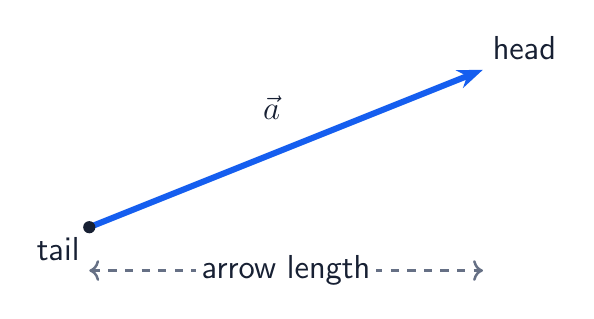
\begin{tikzpicture}[x=1cm,y=1cm]
  \coordinate (T) at (0,0);
  \coordinate (H) at (5,2);
  \draw[mech primary,-{Stealth[length=3.2mm,width=2.4mm]},line cap=butt] (T) -- (H);
  \fill[mechInk] (T) circle (2.2pt);
  \node[below left] at (T) {tail};
  \node[above right] at (H) {head};
  \node[above left] at (2.55,1.25) {$\vec a$};
  \draw[mech guide,<->] (0,-0.55) -- node[fill=white,inner sep=2pt] {arrow length} (5,-0.55);
\end{tikzpicture}
\end{document}
